%!TEX program = xelatex
%
% ================================================================
%	Tipo de dissertação:
%		escolher entre "doutoramento" ou "mestrado"
%
%	Área científica:
%		escolher entre
%			- "ct" (ciências e tecnologia, final); "ctR" (ciências e tecnologia, rascunho);
%			- "csh" (ciências sociais e humanas, final); "cshR" (ciências sociais e humanas, rascunho);
%			- "artes" (artes, final); "artesR" (artes, rascunhos)
%
% ================================================================
%
\documentclass[mestrado,ctR,12pt]{teseue}
%
%
% ================================================================
%	DOCUMENTO:
%		 
%		Língua, Título, Nome do Candidato, Curso, etc
%		Estrutura
% ================================================================
%
% ----------------------------------------------------------------
%
%	LÍNGUA DA TESE
%
%	Opções atuais:
%	- PT: Português (novo acordo ortográfico)
%	- EN: Inglês
%
\tueLINGUA{EN}
%
% ----------------------------------------------------------------
%
%	TÍTULO DA TESE
%
%	Em Português e Inglês.
%
\tueTITULO
{Identity Management in Healthcare Using Blockchain Technology}
{}
%
% ----------------------------------------------------------------
%
%	SUBTÍTULO DA TESE
%
%	Em Português e Inglês.
%
\tueSUBTITULO
{}
{}
%
% ----------------------------------------------------------------
%
%	CANDIDATO
%
%	Nome completo.
%		
\tueCANDIDATO
{João Pedro Nunes dos Santos}
%
% ----------------------------------------------------------------
%
%	TÍTULO E NOME DO/A ORIENTADOR/A
%
%	Designação oficial e nome do orientador/a.
%	Em geral, "Orientador" ou "Orientadora".
%
\tueORIENTADOR
{Orientador}
{Pedro Salgueiro}
%
% ----------------------------------------------------------------
%
%	SEGUNDO ORIENTADOR/A (se aplicável)
%
%	Designação oficial e nome do segundo orientador/a.
%	Em geral, "Co-orientador" ou "Co-orientadora".
%
\tueSEGUNDOORIENTADOR
{Orientador}
{Vítor Beires Nogueira}
%
% ----------------------------------------------------------------
%
%	TERCEIRO ORIENTADOR/A (se aplicável)
%
%	Designação oficial e nome do terceiro orientador/a.
%	Em geral, "Co-orientador" ou "Co-orientadora".
%
%\tueTERCEIROORIENTADOR
%{Co-Orientador}
%{António Inácio Norberto}
%
% ----------------------------------------------------------------
%
%	CURSO
%
%	Nome do curso em que se enquadra esta tese.
%
\tueCURSO
{Engenharia Informática}
%
% ----------------------------------------------------------------
%
%	ESPECIALIDADE (se aplicável)
%
%	Nome da especialidade em que se enquadra esta tese.
%
%\tueESPECIALIDADE
%{Coordenação de Recursos Naturais}
%
% ----------------------------------------------------------------
%
%	DEPARTAMENTO
%
%	Departamento anfitrião do curso.
%
\tueDEPARTAMENTO
{Departamento de Informática}
%
% ----------------------------------------------------------------
%
%	ESCOLA
%
%	Escola a que pertence o departamento.
%
\tueESCOLA
{Escola de Ciências e Tecnologia}
%
% ----------------------------------------------------------------
%
%	PALAVRAS CHAVE
%
%	Data de submissão da tese.
%
\tuePALAVRASCHAVE
{Blockchain, Saúde, Identidade, Big Data}
{Blockchain, Health, Identity, Big Data}
%
% ----------------------------------------------------------------
%
%	DATA
%
%	Data de submissão da tese.
%
\tueDATA
{\today}
%
% ----------------------------------------------------------------
%
%	DEDICATÓRIA
%
\tueDEDICATORIA
{To My Family}
%
% ----------------------------------------------------------------
%
%	PREAMBULO
%
%	Comandos e definições para o LaTeX que devem estar **antes**
%	do texto do documento.
%
\tuePREAMBULOLATEX{
	\usepackage[figureright]{rotating}
}
%
% ----------------------------------------------------------------
%
%	PREAMBULO
%
%	Texto até à página 1. 
%
%	Por omissão os conteúdos estão definidos nos ficheiros
%		- prefacio.tex
%		- agradecimentos.tex
%		- acronimos.tex
%		- sumario.tex
%		- abstract.tex
%
\tuePREAMBULO {
  \chapter*{Acknowledgements}

Firstly, I want to thank my dissertation advisors, Pedro Salgueiro and Vítor
Beires Nogueira, for being patient with me, for their availability and for
their dedication in this project.

I want to thank my family who helped me finish this project, with their
unending support, words of wisdom and for always pushing me to do better.

I also want to thank my work colleagues, who always supported me, helped me
grow as a professional and person, challenged me to improve, and whom I
consider as a second family.

I need to thank my close friends for always believing in me and for always
being available when I needed the most, showing they are true friends.

Lastly, every person who supported me in some manner, I truly am grateful for
your support.

  %!TEX root = main.tex
\begin{tueACRONIMOS}
	\begin{acronym}[IEEE]
		\acro{EHR}{\emph{Electronic Health Record}}
		\acro{HL7}{\emph{Health Level 7}}
		\acro{DDOS}{\emph{Distributed Denial of Service}}
		\acro{BFT}{\emph{Byzantine Fault Tolerant}}
		\acro{GDPR}{\emph{General Data Protection Rule}}
		\acro{DLP}{\emph{Distributed Ledger Platform}}
		\acro{EVM}{\emph{Ethereum Virtual Machine}}
		\acro{SDK}{\emph{Software Development Kit}}
		\acro{MSP}{\emph{Membership Service Provider}}
		\acro{HLF}{\emph{Hyperledger Fabric}}
		\acro{CA}{\emph{Certificate Authority}}
		\acro{FHIR}{\emph{Fast Healthcare Interoperability Resources}}
		\acro{API}{\emph{Application Programming Interface}}
		\acro{JSON}{\emph{JavaScript Object Notation}}
		\acro{FHIR}{\emph{Fast Healthcare Interoperability Resources}}
		\acro{CIA}{\emph{Confidentiality, Integrity, and Availability}}
		\acro{SHA}{\emph{Secure Hash Algorithm}}
		\acro{TLS}{\emph{Transport Layer Security}}
	\end{acronym}
\end{tueACRONIMOS}

  \begin{tueABSTRACT}

  Bitcoin served as the catalyst for creating a solution to secure digital
  transactions without requiring a trusted third party to be involved. To solve
  this problem, the mechanisms now associated with a Blockchain were
  conceptualized and implemented to serve as the backbone for the Bitcoin
  network. More specifically, it was used as a security tool making Bitcoin a
  more transparent and reliable form of cash, a digital cryptographic currency.
  Even tough Bitcoin ended up not fulfilling its intended purpose as a
  currency, the Blockchain technology has enabled further avenues for
  innovation and creativity.

  Blockchain has since been used as the backbone for various cryptocurrencies
  networks. Some implementations of this technology allow the execution of
  code, also known as "smart contracts". Smart contracts are executed in an
  autonomous manner, with no human intervention. These can be used to solve a
  new set of problems due to their transparent behavior, lack of human
  intervention and distributed nature. 

  Blockchain technology allows the creation of systems that introduce a number
  of benefits over traditional data handling used in today's Healthcare
  Information Systems. Costs and risks associated with these systems can be
  reduced and information can become transparent and trustworthy to all
  participants.
  
  The Hyperledger Fabric Network with true private transactions and advanced
  security mechanisms was used to serve as the basis for the system proposed in
  this dissertation. Moreover, a client application was also created that
  interacts with smart contracts to manipulate the ledger.
  
  The work discussed in this dissertation shows that a Blockchain system based
  on Hyperledger Fabric is suitable for managing patients identity, in
  Healthcare. Even tough the feature set of this Blockchain is very focused in
  privacy and security, some additional measures regarding confidentiality of
  data had to be implemented.  Regardless, a system was built successfully that
  met the requirements. The implementation of this system would provide
  transparency, immutability and additional security for patients and medical
  staff alike. 

\end{tueABSTRACT}

  %!TEX root = main.tex
\begin{tueSUMARIO}

  Lorem ipsum dolor sit amet, consectetur adipiscing elit. Vivamus vitae est
  vitae risus varius malesuada et eget velit. Morbi tincidunt venenatis tellus,
  in volutpat ante varius et. Fusce congue maximus velit ac dignissim. Integer
  hendrerit pharetra libero, at vehicula odio vestibulum eget. Etiam eget
  fringilla leo, sit amet posuere nisl. Aenean at tincidunt felis. Cras rhoncus
  mauris libero, a vestibulum risus faucibus quis. Aenean malesuada vitae nibh
  ut dapibus. Pellentesque vel blandit odio.

  Maecenas massa leo, egestas id augue at, aliquam iaculis leo. Etiam ac lacus
  tempus, malesuada dolor vel, mattis leo. Duis tortor mi, accumsan vitae
  ligula eu, luctus accumsan diam. Etiam venenatis elit non magna aliquam
  eleifend. Phasellus in nunc at arcu iaculis ultrices sed sed ante. Nullam in
  velit a metus convallis vestibulum a vitae turpis. Proin fringilla dui
  tempor, ultrices metus nec, lobortis elit. Sed at posuere augue. Phasellus ac
  massa fringilla, convallis urna nec, aliquet orci. Mauris placerat tellus vel
  scelerisque tempus. Donec lacinia tincidunt mattis. Donec congue, augue sed
  ullamcorper placerat, erat nunc vestibulum tellus, vel consequat sem diam in
  magna. Vivamus ac dolor lacinia magna pharetra maximus. Nulla congue feugiat
  vehicula. Praesent luctus purus ac justo tempor eleifend.

  Nunc eu ex vel ipsum ultrices molestie. In eget sodales turpis. Donec egestas
  facilisis nulla id feugiat. Duis gravida lorem quis porttitor interdum. Sed
  turpis leo, aliquet non metus a, vulputate volutpat ante. Donec neque metus,
  volutpat quis congue non, aliquam sed nunc. Curabitur erat mauris, elementum
  id rhoncus quis, condimentum eu felis. Quisque porta gravida velit a congue.
  Nulla gravida suscipit pulvinar. Sed sed erat ut turpis consequat sagittis.
  Sed scelerisque, massa ac tincidunt rutrum, libero dolor suscipit lorem,
  interdum dignissim massa enim a purus. Aliquam porta orci non urna
  sollicitudin, sed lobortis nibh ullamcorper. Aliquam erat volutpat. Phasellus
  ac purus in massa aliquet ultricies non sit amet justo.

  Quisque placerat lobortis risus. Vestibulum ante ipsum primis in faucibus orci
  luctus et ultrices posuere cubilia Curae; Pellentesque eget odio sed lectus
  sollicitudin consectetur et ornare libero. Aliquam et ullamcorper arcu. Fusce
  mollis euismod purus, vitae auctor quam lobortis eu. Nunc mollis, velit eu
  cursus feugiat, nunc neque pellentesque arcu, a suscipit tellus nunc quis
  quam. Cras diam est, fermentum a rutrum sed, pretium eu tortor.

\end{tueSUMARIO}

}
%
% ----------------------------------------------------------------
%
%	CONTEÚDO
%
%	Texto principal da tese.
%
\tueCONTEUDO  % A partir da página 1
{
	\chapter{Introduction}
\label{introduction}

\begin{quote} 
  \emph{This Chapter introduces the main topics and technologies covered by
  this dissertation. Healthcare and its relationship with technology is
  presented. The current flaws associated with patients identity data
  management are described. The Blockchain technology is introduced as a
  potential solution to some of these problems.} 
\end{quote}

The aim of this dissertation is to create a solution for managing the identity
of patients in the Healthcare environment by using Blockchain technology, and
in turn, evaluate the use of this technology in this specific use case.  Health
is intrinsically linked with technology, as new technologies enable safer and
better treatments. Nowadays, Healthcare organizations store patients data on a
digital format. The Electronic Health Record (EHR) is an abstract concept
representing the patients digitally stored clinical data and their identity in
a medical and clinical context.

Standards are an important aspect to take into account when designing an
information system because they allow interoperability between different
organizations. The Health Level 7 (HL7) Fast Healthcare Interoperability
Resources (FHIR) standard (see Section~\ref{blockchainHealthcare}), is being
built primarily by the Health Level Seven organization. Over the last few
years, it has seen a significant growth in usage. It is also an international
standard with partnerships worldwide. HL7 Portugal is now starting its
operations and is building a community to support this standard in
Portugal~\cite{HealthLevel7}.

Blockchain is often known as the technology behind the Bitcoin cryptocurrency.
Bitcoin depends on two complementary technologies, digital tokens and a
Blockchain, that when orchestrated together facilitate trust, immutability and
resiliency~\cite{Evans2016}.

A Blockchain runs on a network of computers and has a list of records that are
replicated across the participating peers. Blockchain, as we know today, was
conceptualized as the public ledger~\footnote{A ledger is defined as an object
in which items are regularly recorded, originally business activities and money
received or paid, but in reality, it can be used to store any type of record.}
for the Bitcoin cryptocurrency in 2008 by Satoshi Nakamoto~\cite{Nakamoto2008}.
Satoshi Nakamoto is a pen name of, a still unknown to this day, individual or
organization of individuals.

Traditional Healthcare databases and architectures are increasingly vulnerable
and a target to groups of malicious actors that possess the technical expertise
to deny services with Distributed Denial of Service (DDOS) attacks~\footnote{A
Distributed Denial of Service attack is an attempt to make an online service
unavailable by overwhelming it with traffic from multiple sources.} or cause a
data breach~\footnote{A data breach is the intentional or unintentional release
of secure or private/confidential information to an untrusted
environment.}~\cite{mcCoy2018}. 

Making matters worse other problems spring to mind. The data that comprises the
identity of a patient is often fragmented across multiple Healthcare
organizations, in such a way that, to get a true overview of the patients
history and diagnosis there would be a need to merge all the pieces of
information stored in data systems that are hosted in architecturally different
Healthcare information systems. Transparency is also a concern, as a patient
does not currently possess the means to track how his medical data is being
handled.

As more information becomes available, new insights can be extracted by
Healthcare professionals that lead to an overall improvement of the patients
interaction with the Healthcare ecosystem. However, maintaining a high amount
of data secure is a costly and risky matter for every party involved. Security
and privacy are a top concern regarding sensitive data. 

This dissertation provides an insight into the design and implementation of a
Blockchain based system for managing the identity of patients in an Healthcare
setting and its subsequent evaluation. The creation of this system and its
subsequent evaluation could provide interesting conclusions to medical staff as
well as patients, regarding its potential implementation and deployment in the
field.

In this document, different Blockchain implementations are explored to get an
overview of their feature set and focus. Considering a set of defined
requirements a platform is chosen, in order to evaluate the suitability of this
technology in the Healthcare field. More precisely, in
Chapter~\ref{background}, a brief introduction to Blockchain and its most
prominent implementations is presented. The technology is further explored in
Chapter~\ref{blockchain} and a number of real world use cases of this
technology in the Healthcare field are explored.  In Chapter~\ref{development}
a Blockchain platform is chosen in order to build a prototype system to
evaluate the usability of this technology in the Healthcare field. Insight is
given into the system design, implementation. In Chapter~\ref{experiments}, the
system is tested and evaluated. Finally, in Chapter~\ref{Conclusion} some
conclusions are presented and potential future work is discussed.

	\chapter{Background}\label{background}


\begin{quote} \emph{"This project aims to build a Blockchain based system to
  manage the identity of patients and investigating the suitability of creating
  such a system in the Healthcare environment according to objective criteria.
  While Blockchain is not a new concept at this point, it is an evolving
  technology that is being used to solve old problems with new approaches while
  at the same time creating new application fields and challenging old
  conventions and methodologies. This Chapter will provide an overview of this
  technology and some of its most prominent implementations. Finally, some
  context is given to how technology has been helping the Healthcare industry
  to enable better management of their patients identity and how the current
  information systems of Healthcare establishments handle this task."}
\end{quote}

\section{Blockchain Technology}

The concept of Blockchain is abstract. It is a collection of technologies
orchestrated to work together. In this sense the concept can be used to refer
to the Bitcoin's Blockchain, alternative implementations or even forks of the
Bitcoin Blockchain called Altchains~\cite{Lewis2015} that share many
characteristics but may have different features and purposes. It can even
refer to platforms that allow execution of code in an autonomous manner,
exactly as it was programmed, with no human intervention.  A Blockchain is,
generally speaking, a continuously growing list of records being written in
the ledger, a structure where all records are written and stored, that is
constantly being replicated across a network of peers, in opposition to
having a single central record history, making it a good example of a
distributed database, thus avoiding having a single central point of failure
that can be easily targetable~\cite{Barclay2017}.

The purpose of a Blockchain is to maintain integrity in a network of
distributed systems~\cite{Drescher2017}. To fulfill this purpose it uses
cryptographic techniques and digital signatures to not only verify the
authenticity of records but also as a way to manage read or write access to
the network and as proof that a record was written in the ledger and was
never tampered with, creating an immutable history of records, that benefits
various use cases as discussed later in this document.

Unlike a conventional database system running in a server, where only a
single entity keeps a copy of the underlying database, making it centralized
by design, the ledger of the Blockchain is constantly replicated across any
number of participating nodes in the network~\cite{Lewis2015} in a regular
cadence defined at the genesis of the network. In some implementations, not
every participant has the same ability to interact with the ledger and in
this respect a Blockchain can be permissionless or permissioned. Generally
speaking, in a permissionless Blockchain every node of the network can write
in the ledger whereas in a permissioned Blockchain only a select group of
entities have access to writing in the ledger, making the permissioned
version, by default secure, if the entities themselves who manage the network
are considered secure and trustworthy by the participants in the
network~\cite{Lewis2015,Valenta2017}.

But then, how does a permissionless Blockchain maintain security if every
participant in the network has access to writing on it, including potentially
malicious parties?

Given that participating nodes in a public network can belong to different
and often competing parties, there is no implied trust between them, so the
Blockchain needs a mechanism to ensure the integrity of the ledger and
prevent malicious meddling from interested parties and avoiding the need for
a central authority~\cite{Barclay2017}.  Take for example the Bitcoin
Blockchain that uses a peer-to-peer network to avoid the requirement of a
third party being involved in a financial transaction such as a financial
institution or a middle man, which must be trusted with the details of a
transaction to see it through~\cite{Nakamoto2008}.

Consensus is a mechanism employed by the Blockchain to solve this problem.
Even though consensus mechanisms can behave vastly different, depending on
its implementation and purpose, they are at the core a solution to create
immutability and ensure resiliency by ensuring the majority of the network
agrees upon the sequence of events.  For example, in the Bitcoin's Blockchain
case, consensus is reached by the longest chain rule where the longest chain
of blocks not only serves as proof of the sequence of events witnessed, but
as proof that it came from the largest pool of computing power, as it uses a
proof of work (\textbf{pow}) algorithm that relies on brute force to solve a
complex mathematical puzzle, making the longest chain of blocks the one with
the most computing power behind it and therefore agreed upon by the majority
of the network~\cite{Baars2016,Wood2017} making it the most likely to be the
one that represents the sequence of events witnessed.

While the Blockchain, we now know today, was conceptualized as the public
ledger for the Bitcoin cryptocurrency in 2008 by Satoshi Nakamoto and
implemented in 2009, many are now using it as a foundation across many
application areas such as traceability and asset management~\cite{MIT2016}.
Thanks to the roaring success of Bitcoin and the increasingly apparent use
cases that the Blockchain can provide, the public and the various industries
interest in this technological advance is rising and it is quickly becoming a
technological foundation in our economic and social systems~\cite{Zago2018,
Marr2018,Long2018}.

\subsection{Ethereum}

Due to Bitcoin getting extensive media coverage, the average public awareness
in cryptocurrencies is shown to be rising~\cite{BitAwareness2017}. While
Blockchain is used as a means to increase the resiliency of the Bitcoin
cryptocurrency from malicious parties, a token is used to represent the coin. 

Just like a Dollar it has no value by itself, it has value only because we
agree to trade goods and services in exchange for a higher amount of the
currency under our control and we believe others will do the same
\cite{aliessi2016}. Through the years Blockchain has evolved to be capable of
being an independent development platform using the token as a means to
reward those who maintain the consensus by spending electricity and
computation power in the network. In some networks like Ethereum one can
build upon the network to create Decentralized Applications (\textbf{Ðapps})
that allow logic to be executed in an autonomous manner~\cite{Wood2017}. 

In the same manner that the Bitcoin Blockchain can be seen as an adding
machine, the Ethereum Blockchain can be seen as a computer able to execute
programs designed for it~\cite{Wood2015}.

Ethereum is an open-source platform based on the Blockchain technology that
enables developers to build and deploy \textbf{Ðapps}. Ethereum is being
developed by the Ethereum Foundation and was first discussed by Buterin in
2013.  Ethereum intends to provide a Blockchain with a built-in programming
language that is used to create \textit{Smart contracts}~\cite{Wood2017}.

These are used to describe the logic of any system that developers can
imagine and, when created, can be deployed to the Blockchain where they
execute as “autonomous agents”.  Thanks to these tools it is safe to say that
long gone are the days where building Blockchain applications required a
complex background in coding cryptography, mathematics as well as significant
resources~\cite{Wood2017,BlockGeeks2017}.

The Ethereum Blockchain is a permissionless Blockchain, and thus, it must
have a consensus mechanism to ensure the validation process of every record
and, in turn, ensure resiliency and immutability. While other implementations
of the Blockchain have different consensus mechanics, in Ethereum’s case, all
participants have to reach consensus over the order of all transactions that
have taken place. If a definitive order cannot be established then a
double-spend~\footnote{Double-spending is a potential flaw in a digital cash
scheme in which the same single digital token can be spent more than once.
This is possible because a digital token consists of a digital file that can
be duplicated or falsified. As with counterfeit money, such double-spending
leads to inflation by creating a new amount of fraudulent currency that did
not previously exist. This devalues the currency relative to other monetary
units, and diminishes user trust as well as the circulation and retention of
the currency.} might have occurred and the transaction is
rejected~\cite{Wood2017}.

\subsection{Fabric}

Hyperledger Fabric (\textbf{hlf}) is part of the Hyperledger project started
in December 2015 by the Linux Foundation, and is an open-source
developer-focused community of communities focused on the development of
enterprise-grade, open-source Blockchain-based solutions.  Fabric is an
implementation of a Distributed Ledger Platform (\textbf{dlp}) under the
Hyperledger umbrella~\cite{Cachin2016}.

Hyperledger Fabric’s initial commit was contributed by IBM and written in the
Go programming language.  It is a permissioned Blockchain and its main design
goal was to surpass previous Blockchain implementation limitations, such as,
lack of true private transactions and confidential contracts.

These goals are achieved thanks to assigning peers in the network three
distinct roles and by offering the ability to create channels each with its
own private ledger.  A peer can have the role of endorser, committer or
consenter or sometimes multiple roles.  Hyperledger Fabric is intended as a
foundation for developing applications in a modular fashion, opting for a
plug-and-play approach to its various components as well as its consensus
mechanism~\cite{HyperledgerFabricDocs2017}.

Hyperledger Fabric, as discussed, also allows the creation of smart contracts
which can be written in Chaincode.  Given that this Blockchain's key
operational requirement is privacy, featuring true private transactions and
confidential contracts, it makes this technology a great asset for a business
environment where sensitive information must be handled with care and
disclosed on a case by case basis.  Thanks to its modular approach consensus
protocols are no longer hard-coded and trust models can be repurposed.

\subsection{Burrow}

Hyperledger Burrow (\textbf{hlb}) is also part of the Hyperledger project and
its development started in 2014 by Monax and sponsored by Intel. It is a
permissionable smart contract machine written in Go and offers a modular
Blockchain client with a permissioned smart contract interpreter built, in
part, to the specification of the Ethereum Virtual Machine (\textbf{evm})
with the client having, essentially, three main components, the consensus
engine, the permissioned \textbf{evm} and the Remote Procedure Call
(\textbf{rpc}) gateway~\cite{Kuhlman2017,HyperledgerBurrow2017}.

Hyperledger Burrow has its own Consensus Engine, the Byzantine fault-tolerant
Tendermint protocol.  The Tendermint protocol is an open-source effort that
allows high performance in solving the consensus problem and also has a
flexible interface for building arbitrary applications above the consensus,
as well as, a suite of tools for deployments and their
management~\cite{Buchman2016}.

\section{Identity in Healthcare}

Originally records of a patient were stored in paper, a physical format.
Thanks to the advent of the computers more and more records are stored on a
digital format and the Electronic Health Record (EHR) was created.
\cite{Marquez2017}  This benefits handling of information between the patient
and the medical professionals and medical
institutions.\cite{ONCoordinator2017} But first we must discuss what is
defined as identity in this specific case.

Identity is a construct that depends on the context.  Identity can be defined
as the characteristics determining who or what a person is.  In this paper we
define identity as the set of characteristics that determine who is the
patient in the given Healthcare ecosystem they belong to, such as, the name,
the age, the cellphone number, the gender and the birth date of the patient.
Electronic Health Records encapsulate this information in digital format,
however, they are usually represented in a format according to the
Information System they were designed to work with.

To enable interoperability, standards for EHRs were created and many failed
to bring the much needed consensus that was required for interoperability
between different Information Systems in different institutions.
\cite{Eichelberg2006} Health Level 7 has done much work to be recognized in
many countries and is quickly being implemented in many countries to allow
for joint efforts between organizations. \cite{HL7Anual2016}

Even with these advances in mind, the nature of many clinics and hospitals
Information Systems makes the management of their patients identity a very
cumbersome, costly and risky affair to handle.  Security in a connected age,
where internet is easily available, is lagging behind and presenting some
problems.  There is also the question of transparent use of information by
the organizations that store it.

	\section{Identity in Healthcare}

Originally records of a patient were stored in paper, a physical format.
Thanks to the advent of the computers more and more records are stored on a
digital format and the Electronic Health Record (EHR) was created.
\cite{Marquez2017}  This benefits handling of information between the patient
and the medical professionals and medical institutions.\cite{ONCoordinator2017}
But first we must discuss what is defined as identity in this specific case.

Identity is a construct that depends on the context.  Identity can be defined
as the characteristics determining who or what a person is.  In this paper we
define identity as the set of characteristics that determine who is the patient
in the given Healthcare ecosystem they belong to, such as, the name, the age,
the cellphone number, the gender and the birth date of the patient.  Electronic
Health Records encapsulate this information in digital format, however, they
are usually represented in a format according to the Information System they
were designed to work with.

To enable interoperability, standards for EHRs were created and many failed to
bring the much needed consensus that was required for interoperability between
different Information Systems in different institutions. \cite{Eichelberg2006}
Health Level 7 has done much work to be recognized in many countries and is
quickly being implemented in many countries to allow for joint efforts between
organizations. \cite{HL7Anual2016}

Even with these advances in mind, the nature of many clinics and hospitals
Information Systems makes the management of their patients identity a very
cumbersome, costly and risky affair to handle.  Security in a connected age,
where internet is easily available, is lagging behind and presenting some
problems.  There is also the question of transparent use of information by the
organizations that store it.

	\chapter{Blockchain: A Practical Overview and Use Cases}\label{blockchain}

\begin{quote} 
  \emph{It was for a long time necessary, to establish trust between two
  entites, a middle-man with a netral stake. The blockchain aims to solve this
  depency using decentralization and a mechanism called consensus. A Blockchain
  is a distributed system which means that processing is shared across multiple
  nodes. Permissioned Blockchains are more suited towards enterprise and
  organizations while still benefiting from the immutability of the Blockchain
  architecture. Ethereum is a permissionless implementation whereas Fabric is
  Permissioned. Ethereum uses a currency to maintain the network while Fabric
  uses \textbf{BFT} consensus which does not need a currency. Both feature
  smart contracts even tough they feature different execution architectures.
  Ultimately, the Hyperledger Fabric Distributed Ledger Platform , with its
  focus on enterprise use and true data segregation, was chosen as the platform
  to build a system that seeks to achieve the purpose mentioned in
  Chapter~\ref{introduction}.}
\end{quote}

The Blockchain, initially used to solve problems in centralized financial
systems, has inherent characteristics that make it suitable for a variety of
use cases. This Chapter will provide a more practical exploration of the
Blockchain technology showing some of the considerations that were taken into
account, after analyzing some implementations of this technology, mentioned in
Chapter~\ref{background}.

\section{Trust in a Network}

Blockchain implementations are an emerging structure for distributed computing
systems that provide an immutable history of records written to a ledger, even
when there is no implicit trust relationship between the parties
involved~\cite{Barclay2017}.

Banks used to keep track of their financial transactions by writing on a book
usually located at the central bank. This book was often called ledger.
Whenever a transaction occurred someone wrote on the book. In short, the ledger
acts as a mean of storing all the transaction details between the bank and
other entities. 

Nowadays banks do not use the ledger in a book format. Instead the ledger is
referred to as the structure that holds all transaction information the bank
possesses. It is a structure that keeps the original purpose of recording all
the transactions that are made.

Imagine the following situation- Joe is on vacation and needs to borrow money
from Jane, his wife. Joe calls Jane to ask for some money and Jane tells him it
will send the money right away. Jane then proceeds to call her account manager
to transfer some of her money to Joe. Finally Jane calls Joe to tell him that
she made the request to send money to him.  As seen on
Figure~\ref{fig:centralizedvsdescentralized} Joe and Jane need to use and trust
the account manager and the bank as a middle man in order to complete this
transaction. If the bank was ever to be unavailable, the bank's database was
corrupted or if someone with  privileged access was able to intercept the
transactions from inside the bank then all transactions between Joe and Jane
would fail creating additional costs to all parties involved. 

\begin{figure}[h]
  \centering
  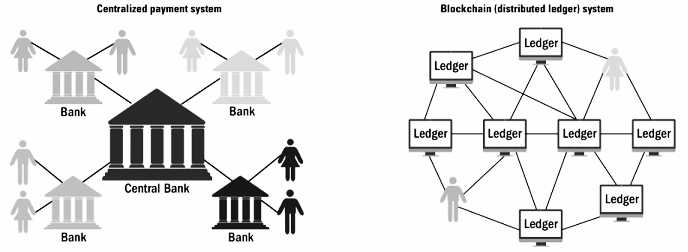
\includegraphics[width=1\linewidth]{imgs/blockchainvscentralizedNetwork.png}
  \caption{\label{fig:centralizedvsdescentralized} A comparison between a
  Centralized Banking System and a Distributed Ledger. (Source: Finance \&
  Development, 2016)}
\end{figure}

It was for a long time necessary, to establish trust between two entities, a
middle-man with a neutral stake. While the ledger is also at the core of the
Blockchain, this technology aims to solve the dependency placed upon third
parties using decentralization and aims to make two different entities trust
each other through constant replication of the ledger, a security mechanism
called consensus.  While consensus has a system performance impact due to the
necessary replication of data, it is a mechanism that establishes a set of
rules that defines if a sequence of transactions is considered valid.
Different Blockchain implementations often use a variety consensus protocols to
balance this trade-off.

\section{Permissionless and Permissioned Blockchain Implementations}


There are three types of computer systems, as seen on Figure
\ref{fig:typesofnetworks}. As previously mentioned in this Chapter, Blockchain
was created out of a desire to solve problems that are displayed in the
centralized financial systems that society is currently based upon.

\begin{figure}[h]
	\centering
	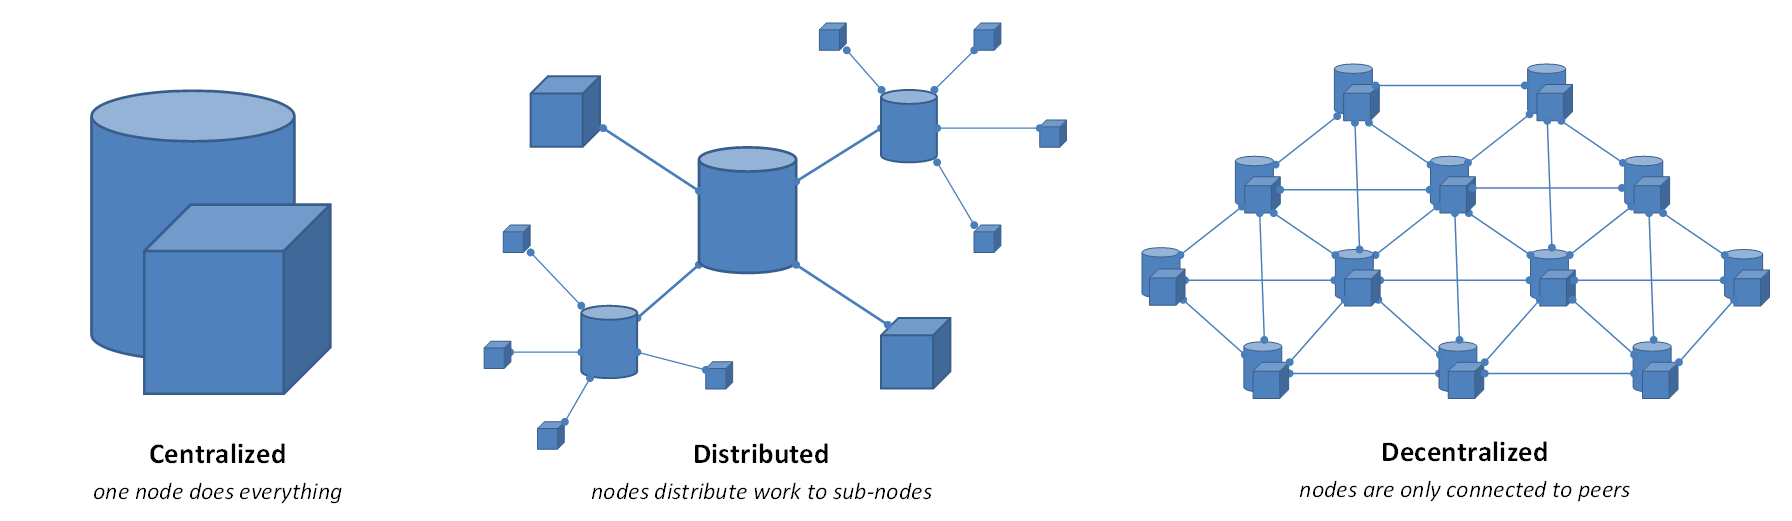
\includegraphics[width=1\linewidth]{imgs/typesofnetworks.png}
  \caption{\label{fig:typesofnetworks} A comparison between different types of
  systems. (Source: Eric Grange, 2016)}
\end{figure}

Put simply, a centralized system is one that is governed by a hierarchical
authority; examples of such being banks, credit card company’s, etc. If you
want to use a Visa card you must request access from Visa and be approved. At
any time your access to that line of credit and your funds may be made
unavailable to you and your access permanently revoked~\cite{Dreifuerst2018}.

In contrast, distributed systems are based upon the philosophy that processing
is shared across multiple nodes even if the decisions themselves may still be
centralized and use complete system state knowledge of the network. Finally, a
decentralized system is one where no single node can make a decision
individually, instead relying on the other participants to reach an agreement
and make a decision, as no single node has a complete system state knowledge.
With this in mind, a decentralized system is seen as a subset of a distributed
system.

A Blockchain is a distributed by design. However there are two major
implementation categories as discussed briefly on Chapter~\ref{background}.

Permisionless Blockchain implementations were the first to appear and while
some industries saw benefits in using the technology, some saw drawbacks to
adopting it in enterprise-grade systems~\cite{Gopinath2016} due to this
unregulated nature. They do have some advantages however compared to
traditional systems.

\textbf{Permisionless} Blockchain implementations, like the Bitcoin's and
Ethereum's Blockchain for example, have no barrier to entry. This means that
anyone can, in theory, participate in the network, write into it as a result of
mining and store data in the ledger sharing the work needed to maintain the
network.  Permisionless implementations have some strengths. These are
completely open and transactions are transparent while also being able to offer
anonymity or pseudo-anonymity. They also take away the need for system
administrators or central servers since the network is based exclusively on
peer-to-peer technology and decisions are made by every participant, creating
reduced costs to maintain and deploy \textbf{Ðapps}. On the other hand, these
implementations are slower than traditional systems because every node must
participate in consensus creating an overhead before a transaction is
considered verified. Due to this there is also a time cost associated because
of the need to wait until verification of the transaction. They operate without
clear legal rules and are trust-free, meaning that there is no responsible
entity if data loss or damages affect systems based on this implementation.

\textbf{Permissioned} Blockchain implementations have some clear advantages for
enterprise. They are faster because consensus is done by a set of nodes instead
of the entire network, can fall back on the legal system because it features an
identity service. This means the platform is auditable and that there is a
legal responsible entity or entities that manage the network. However, costs
when compared to the permissionless variant are higher due to having the need
for a system administrator and servers to manage the network, featuring a
private membership meaning that they are closed to the general public and
managed by a set of entities and are a compromise between the original vision
of a completely decentralized network and enterprise needs and concerns. 

Enterprises benefit greatly from the immutability of the Blockchain
architecture, in that all records cannot be changed. By adding authorized
identity services onto Blockchain, they can meet the regulatory needs of their
industries, by allowing the network to be auditable and assets to be traceable,
falling back to laws or regulations if a dispute between participating entities
occurs~\cite{Barclay2017}.

\section{A Decentralized Open Platform - Ethereum}

Ethereum is a permissionless Blockchain implementation. It is a platform that
lets anyone build and use decentralized applications commonly named
\textbf{Ðapps}. It is an open-source project developed primarily by the
Ethereum Foundation and was designed to be adaptable and flexible, in contrast
to Bitcoin's Blockchain that only records financial
transactions~\cite{EthereumDocs2018}.

It features a friendly programming language called Solidity that is influenced
by C++, Python and Javascript that is designed to allow an easy way for
developers to create new applications on the Ethereum platform with code of
arbitrary algorithmic complexity in a turing complete language. Smart Contract
application code targets the Ethereum Virtual Machine, which is then deployed
to the Blockchain via a local Ethereum node~\cite{Wood2017,Barclay2017}.

At the heart of Ethereum is the Ethereum Virtual Machine (\textbf{EVM}) as seen
on Figure~\ref{fig:evm} and, like any Blockchain, Ethereum also includes a
peer-to-peer network protocol. The Ethereum Blockchain database is maintained
and updated by many nodes connected to the network. Each and every node of the
network runs the \textbf{EVM} and executes the same instructions in order to
maintain consensus across the entire Blockchain. Decentralized consensus gives
Ethereum a high degree of fault tolerance, ensures zero downtime, and makes
data stored on the Blockchain forever unchangeable and
censorship-resistant~\cite{EthereumDocs2018}.

\begin{figure}[h]
  \centering
  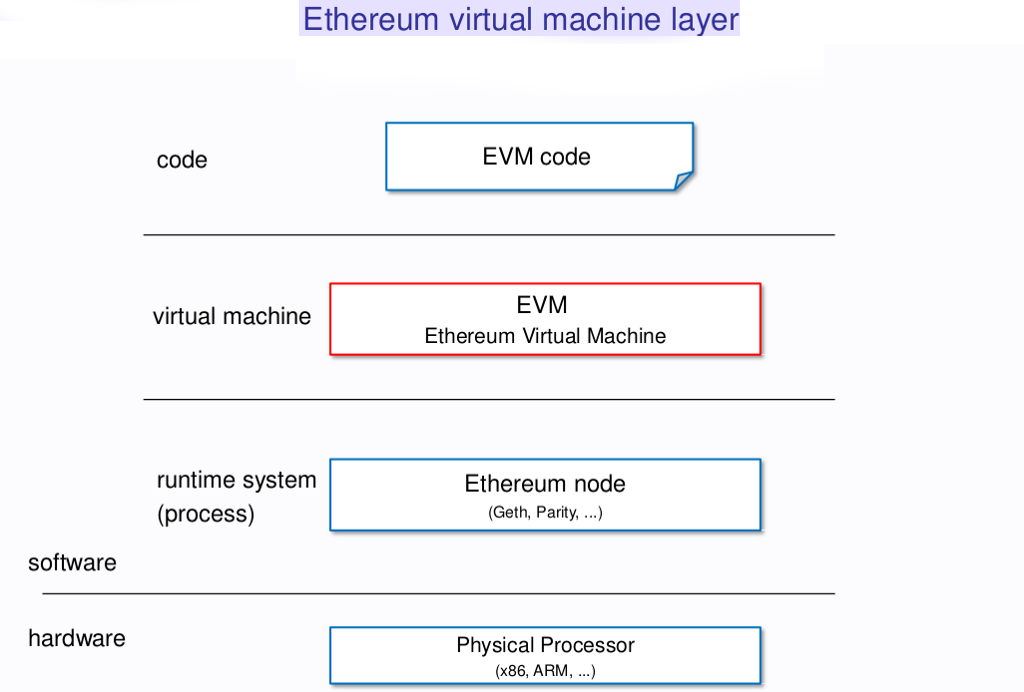
\includegraphics[width=1\linewidth]{imgs/ethereumVirtualMachine.png}
  \caption{\label{fig:evm} A diagram of where \textbf{EVM} fits into the
  Ethereum Platform (Original: Vaibhav Saini, 2018)}
\end{figure}

Users must pay a small transaction fee to the network each time they execute a
transaction. This protects the Ethereum Blockchain from frivolous or malicious
computational tasks, like Distributed Denial of Service (\textbf{DDOS}) attacks
or an infinite loop in smart contract logic. The sender of a transaction must
pay for each step of the “program” they activated, including computation and
memory storage. These fees are paid in amounts of Ethereum’s native
value-token, ether, and then these transaction fees are collected by the nodes
that validate the network commonly called miners - which are nodes in the
network that receive, propagate, verify, and execute transactions. Ethereum
currently uses a proof of work (\textbf{POW}) based consensus algorithm but
plans to change to a proof of stake (\textbf{POS}) algorithm due to
environmental and financial concerns as well as reduced centralization
risks~\cite{EthereumDocs2018,EthereumPOSFAQ2018}.

Ethereum has a live production network called “mainnet” available for any
developer to deploy applications to, as well as three test networks. "Ropsten”
is based on a \textbf{POW} algorithm while "Rinkeby" and "Kovan" are based on a
Proof of Authority~\footnote{In Proof of Authority based networks, transactions
and blocks are validated by approved accounts, known as validators. Validators
run software allowing them to put transactions in blocks. The process is
automated and does not require validators to be constantly monitoring their
computers. It does, however, require maintaining the authority node
uncompromised.} (\textbf{POA}) and all of them are publicly available and free
to use~\cite{Barclay2017,EthereumTestNetworks2018}.

Ethereum has had some unforeseen problems along the way, namely the
\textbf{DAO} heist where a hacker took advantage of a bug in a smart contract
to steal a great sum of money. With Ethereum frequently reaching full
transaction capacity, scaling solutions are the next big
investment~\cite{ethereumScalability2018}.

There are a few proposed solutions by Buterin. For example, \textbf{sharding}
is a solution that aims to avoid every node processing all data in order to
verify and process a transaction. When transactions are initiated they will not
be directed to all the nodes but would instead only be directed to those
depending on the shard in question.  Another solution is off chain computation
where a layer apart from the Blockchain is created and where all the
computation or solving of a complex mathematical equation takes place. This
would not only take the load off the Ethereum Blockchain but also help decrease
the cost of transaction verification and processing. This mechanism would
ensure that the tasks that account for slower transaction speeds on the
Ethereum’s Blockchain do not affect the whole network. Finally, to avoid every
node having the need to download the entirety of the Blockchain's data, the
complete picture can be stored on cloud and each node only has to store and
load relevant data~\cite{ethereumBlogScalability2018}.

\section{A Permissioned Distributed Ledger Platform - Hyperledger Fabric}
\label{distributedLedgerPlatform}

Hyperledger Fabric is a platform for distributed ledger solutions featuring a
modular architecture. It provides developers with a permissioned platform
targeted at business and enterprise use cases that supports pluggable
implementations of different components to accommodate the complexity and
intricacies that exist across the economic ecosystem. It is an open source
project initially commited by IBM  and estabilished under the Linux Foundation,
being developed by over 44 organizations and more than 250
members~\cite{HyperledgerFabricDocs2017,HyperledgerGrowth2018}.

It supports the creation of smart contracts, commonly called "chaincode" in
Fabric, that are authored in general-purpose programming languages such as
Java, Go and Node.js rather than constrained domain-specific languages
(\textbf{DSL}). 

Chaincode in Fabric consists of two components - the code itself, which
describes the logic of the program running in the execution phase, and the
endorsement policy that describes how a specific chaincode transaction is
validated. For example, a typical endorsement policy lets the chaincode specify
the endorsers for a transaction in the form of a set of peers that are
necessary for endorsement and subsequent successful
validation~\cite{Androulaki2018}. Chaincode runs in a container isolated from
the peer process which consented its installation providing aditional control
over information dissemination.

At the heart of Fabric is the permissioned distributed ledger that provides a
way to secure the interactions among a group of entities that have a common
goal but which may not fully trust each other. By relying on the identities of
the participants, a permissioned ledger platform can use a more traditional
crash fault tolerant (\textbf{CFT}) or byzantine fault tolerant (\textbf{BFT})
consensus protocols that do not require mining or an associated currency in
order to achieve consensus.

\begin{figure}[h]
  \centering
  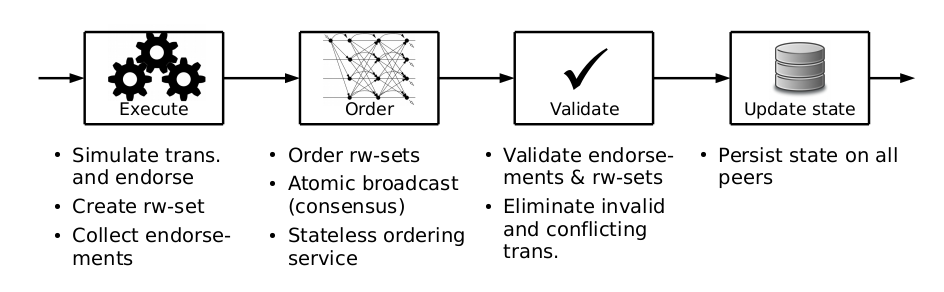
\includegraphics[width=1\linewidth]{imgs/executeOrderValidate.png}
  \caption{\label{fig:executeorder} Execute-order-validate architecture of
  Fabric (Source: IBM, 2018)}
\end{figure}

Fabric introduces the execute-order-validate Blockchain architecture as shown
on Figure~\ref{fig:executeorder} and does not follow the standard order-execute
design illustrated on Figure~\ref{fig:orderexecute} \cite{Androulaki2018}. In
this architecture, when a client sends transactions to the peers specified by
endorsement policy. Each transaction is then executed and its output is
recorded. After execution, transactions enter the ordering phase. An ordered
sequence of transactions grouped into blocks are produced using the consensus
mechanism. Then, these blocks are broadcast to all peers. Fabric orders the
transaction outputs computed during the execution phase. Each peer then
validates state changes according to the endorsement policy and the consistency
of the execution in the validation phase. All peers validate the transactions
in the same order and validation is deterministic. In this sense, Fabric
introduces a novel hybrid replication paradigm in the Byzantine
model~\cite{Androulaki2018}. This model combines passive replication, which is
the pre-consensus computation of state updates, with active replication, the
post-consensus validation of execution results and state changes.

\begin{figure}[h]
  \centering
  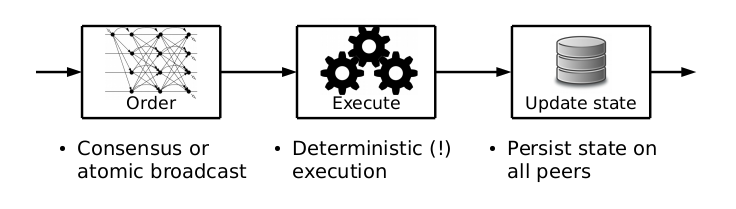
\includegraphics[width=0.8\linewidth]{imgs/orderExecuteArchitecture.png}
  \caption{\label{fig:orderexecute} Order-execute architecture in Replicated
  Services Like Ethereum (Source: IBM, 2018)}
\end{figure}

On the other hand, the order-execute architecture is conceptually simple,
leading it to be currently widely implemented in replicated services such as
Blockchain. In this architecture the transactions are executed sequentially on
all peers which limits the maximum number of simultaneous transactions that can
be achieved.  Additionally a Denial of Service (\textbf{DOS}) attack can be
mounted just by deploying a slow performing smart contract or one with an
infinite loop to the network since the Blockchain forms a distributed computing
engine.  To cope with this issue, public programmable Blockchains with an
associated cryptocurrency, account for the execution cost of executing of the
program.

In Fabric all nodes that participate in the network have an identity, as
provided by a modular Membership Service Provider (\textbf{MSP}).  A
\textbf{MSP} is a component that aims to offer the abstraction of a membership
operation architecture meaning that all identities are only allowed to
participate if verified to be considered trustworthy.  The \textbf{MSP}
maintains the identities of all nodes in the system and is responsible for
issuing credentials that are used for node authentication and authorization. An
\textbf{MSP} may define their own notion of identity, and the rules by which
those identities are governed and authenticated using signature generation and
verification~\cite{HyperledgerFabricDocs2017}.

Fabric also assigns different roles to peers. Nodes in Fabric network can have
one or more, of these three roles:

\begin{itemize}
  \item Clients submit transaction proposals for execution, help orchestrate
    the execution phase, and broadcast transactions for ordering.

  \item Peers execute transaction proposals and validate transactions.  All
    peers maintain the ledger, where all transactions  are recorded in the form
    of a hash chain, as well as the state, a succinct representation of the
    latest ledger state. Not all peers execute all transactions.

  \item Ordering Service Nodes (\textbf{OSN}) or orderers are the nodes that
    collectively form the ordering service. In short, the ordering service
    establishes the total order of all transactions in Fabric, where each
    transaction contains state updates and dependencies computed during the
    execution phase, along with cryptographic signatures of the endorsing peers
    defined in the endorsing policy of the transaction. Orderers are entirely
    unaware of the application state, and do not participate in the execution
    nor in the validation of transactions. This design choice renders consensus
    in Fabric as modular as possible and simplifies the replacement of
    consensus protocols in Fabric. 
\end{itemize}

Looking ahead, Hyperledger Fabric will continue to focus on privacy and
confidentiality with v1.2 being recently released, v1.3 and 1.4 expected to be
out this year with further emphasis on these aspects in a regular quarterly
cadence~\cite{hyperledgerRoadmap2018}.

	\chapter{Designing and Building the System} \label{development}

\emph{In this Chapter requirements for a system built upon Blockchain
technology were set. The requirements where chosen in order to create a system
that is interesting to an organization while still respecting the patients data
and their access right to it. With the requirements set, Ethereum and
Hyperledger Fabric advantages and disadvantages were weighted for this use
case. Ultimately, the Hyperledger Fabric Distributed Ledger Platform , with its
focus on enterprise use and true data segregation, was chosen as the platform
to build a system that seeks to achieve the purpose mentioned in
Chapter~\ref{introduction}. A working knowledge of the Fabric platform was
acquired. A Fabric network is comprised by the ledger, the peers, the
applications and the Membership Service Provider and CA provider. To test this
system a network was created to test the interaction possibilities between a
patient and a doctor, translating into two organizations and two peers. Some
tests were executed and the system was evaluated against the Confidentiality,
Integrity and Availability triad model. Symmetric key encryption was required
to be implemented in order to fulfill the confidentiality requirement set.
After these changes a system was implemented that successfully met the
requirements and further conclusions were able to be taken.}

The goal of this thesis is to evaluate the suitability of Blockchain technology
in managing the identity of patients in an Healthcare organization by
conceptualizing and implementing a system that fulfills this role. In order to
fulfill this goal, the development part of this thesis was primarily divided
into four steps with each step building upon the previous ones. This Chapter
provides an insight into the workflow used to build the system. The workflow
spans the conceptualization and its associated challenges and ends in the
implementation of said system. This system was built using some of the
technologies and concepts described in the previous section.

\section{First Step - Defining Requirements and Choosing a
Platform}\label{choosingHyperledger}

After investigating the various Blockchain platforms some criteria was needed
to serve as reference. As such, the first step consisted in defining a set of
key points that the built system had to fulfill. Defining the requirements
proved helpful to choose the most appropriate platform for the objectives as
explained later.

\subsection{Requirement Definition} 
The requirements for this work were deemed to be as follows:

\renewcommand{\labelenumi}{\Roman{enumi}.}
\begin{enumerate}
  \item The system must allow a patient to opt into the network and register as
    a participant.
  \item The system must allow a patient to record his medical data under the
    approval of an administrator.
  \item The system must keep information confidential, transparent and have
    high availability.
  \item The system must provide the patient with the ability to share his data
    with another entity participating in the network, for example sharing
    information with a doctor.
  \item The system must allow the deletion of a patient's data in some manner,
    if he wishes to do so, in order to comply with European privacy laws,
    discussed in Section~\ref{blockchainHealthcare}.
\end{enumerate}

These requirements were chosen in order to create a system that is interesting
to an organization while still respecting the patients data and their access
right to it. 

After defining the requirements it was nececessary to choose the Blockchain
platform that best fulfills these requirements.

\subsection{Choosing a Platform}\label{choosePlatform}

Even tough Blockchain platforms normally originate from the realization that
full centralization has major drawbacks they often have different goals
translating in architecture differences and different development focus.  These
range from open networks, such as Ethereum which anyone can join and use, to
permissioned distributed ledgers, which can be run publicly or privately but
are only open to access and participation through a membership service, such as
Hyperledger Fabric and Hyperledger Indy.

Ethereum is a popular platform on its own right and has certainly paved the way
for Blockchain to be used as a platform that can be extended and built upon. It
has a growing learning ecosystem and community. It is easy to start interacting
with the network as anyone is able to simply download a client and connect to
it.  Thanks to the Solidity smart contract language being targeted for the
specific purpose of authoring smart contracts it only allows for a
deterministic program to be written avoiding potential conflicts in the
execution of these, for example, in the production network. Also after the
initial learning barrier of it being a Domain Specific Launguage it becomes a
platform easy to develop for since it provides a well thought out and well
organized documentation with a easy to use library of operations.

Ethereum is being used in a great deal of projects around the world proving its
stability and suitability in a wide variety of use cases. On the other hand,
handling patients medical data is a great responsibility due to the private and
personal nature of this data. Also hospitals and Healthcare clinics must obey
the regulatory laws regarding privacy and usage of this data.

It is also worth noting that while Ethereum can handle private data exchange by
building upon it, as shown by Barclay, it was not designed with this intent in
mind, therefore these middle ground solutions can prove to be unwise to use at
scale given Ethereum's and the whole Blockchain's ecosystem past problems with
scalability.  

Fabric, like Ethereum, was built with the intention of being a general purpose
use Blockchain. It provides developers with the tools needed to build any
system they can imagine. However, the latter is clearly focused on making
organizations feel more at ease by being auditable as it offers an identity
service and a known environment due to using a membership service provider,
using a private certificate authority that emits certificates specific for the
Fabric network. These concerns allow this platform to avoid the same fate
Internet of Things devices have had in the Healthcare field~\cite{Tana2017}.
The lack of security regulations and ambiguity in how data was being collected
by these devices has limited their usage and prevented the widespread usage of
these devices in the Healthcare field.

Fabric also has good amount of development tools that are now maturing and a
good learning environment with ample documentation about every aspect important
for a developer looking to get started into it. Fabric is being backed by the
Linux Foundation and IBM, lending credibility to the project and ensuring that
this platform is supported and developed into the foreseeable future, as it is
being governed by a diverse technical steering committee and by a diverse set
of maintainers from multiple organizations. In regards to performance the focus
in this area is clear as the Hyperledger community has appointed a Performance
and Scale working group to improve performance as well being tasked to
implement benchmarking framework for Hyperledger projects called Hyperledger
Caliper~\cite{performanceScale2017}.

Regarding Fabric's features, it lends itself very well to fulfill the project
requirements. Fabric's channels and private data segregation at peer level make
a clear statement that privacy is important in this platform which is in line
with the requirements that were laid out for this project. It is also worth
noting that many upcoming Blockchain based projects in the Healthcare field are
using permissioned networks due to these same concerns regarding the privacy of
the patients while retaining the key benefits of Blockchain such as
immutability and decentralization. The fact that Fabric has no associated
currency also means there is no required mining incentives to maintain the
network, even tough it does require some additional infrastructure acquisitions
to set up the network, leading to a higher initial investment in a solution
based on this platform.

Both are very interesting platforms, but ultimately it was decided to use
Hyperledger Fabric as the platform on which to build upon. This decision was
taken in part because Fabric was purpose built for a very regulated environment
and is focused on privacy and scalability which are required in the Healthcare
field. Also, this technology is relatively recent and there is still a great
lack of knowledge available to the general public, making it a more interesting
choice from an theoretical standpoint.

\section{Working knowledge of the Platform}

After choosing to work with Hyperledger Fabric it became necessary to
understand in further detail what are the components that form a network and
the tools to manage these components. This section discusses the main
components of a Fabric network and the tools required to create and maintain a
Fabric network. These components often interact with one another and provide
the technical infrastructure that comprises this technology.

\subsection{Hyperledger Fabric Components}

An Hyperledger Fabric (HLF) network is defined as the technical infrastructure
that provides ledger and smart contract services to applications. Smart
contracts are used to generate transactions and interact with the ledger. The
network is comprised of several components as presented shortly.

The ledger is a central component of a HLF network. The ledger is composed by a
world state and a Blockchain. The world state is a database that holds the
current values of ledger states. States are, by default, expressed as key-value
pairs. The world state is useful because it makes it easy for a smart contract
to get the current value of these states, instead of having to traverse the
entire transaction log. The Blockchain holds the transaction logs that record
the history of changes that have resulted in the current world state.
Transactions are collected and recorded in an immutable sequence of blocks, in
which each block contains a set of ordered transactions by the orderer service.

Another component is the set of peers participating in the network. A Peer is a
node that hosts a copy of the multiple ledgers and smart contracts. There is
one logical ledger in a Hyperledger Fabric network, even tough in reality, the
network maintains multiple copies of a ledger that are synchronized through
consensus. HLF opts to allow multiple ledgers in a network to achieve different
goals of a greater purpose. This allows the creation of channels of information
between trusted parties, for example, a channel of secure and private
information between the clinical staff of an hospital and a patient as
discussed on Chapter~\ref{background}, in which every channel has a ledger.

Through a peer connection, applications execute chaincode that queries or
updates a ledger. Peers have at least one of the three different roles assigned
to them, as seen on Section~\ref{distributedLedgerPlatform}. Applications
always connect to peers when they need to access ledgers and smart contracts.
Every peer in the network is assigned a digital certificate by an administrator
from its owning organization. The mapping of a peer's identity in an
organization is provided through the membership service provider. 

In fact peers, applications, end users (clients), administrators, channels and
organizations must have an identity provided by the MSP in order to be able to
interact with the network. Each of these actors has a digital identity
encapsulated in an X.509 digital certificate standard which must be unique to
every entity. These determine the exact permissions these have over resources
and access to information in the network. The MSP issues these certificates
through the built-in CA component, the Fabric Certificate Authority (CA). The
Fabric CA is a private root CA provider that consists in a CA server and a CA
client. The MSP also supports Certificate Revocation Lists (CRL).

\subsection{Administrating a HLF Networks}


As discussed, a HLF network must have an administrator. HLF provides the
\textit{cryptogen}, \textit{configtxgen}, \textit{configtxlator} and
\textit{peer} tools that are used to configure the network to suit different
needs and use cases.

The \textit{cryptogen} tool generates cryptographic data consuming the file
\textit{crypto-config.yaml}.

The \textit{configtxgen} tool generates the genesis block for the orderer
services and the initial transactions.  This tool consumes the file
\textit{configtx.yaml} that defines configuration parameters for channels, the
genesis block and the orderer service.

The \textit{configtxlator} tool is also used to generate channel
configurations.  Finally the \textit{peer} tool is used to manage the
participating peers in the HLF network.

These tools are used to create and maintain the topology of the network and are
invoked when a change to the network is made, for example, when permissions to
certain records are changed or a new user is enrolled in the network and are
very much intertwined with the Fabric Certificate Authority (CA) discussed in
subsection .

\section{Building the System}

After considering the project goals of investigating the suitability of a
Blockchain based system to manage patients in Healthcare, the third step was to
build a prototype of a system that would provide a simulation of the production
network, albeit on a smaller scale. The insights gained from developing a
simple working system would enable benefits and risks of the approach to be
identified, and opportunities for further research to be laid out.

In order to build a solution, the research done before hand was taken into
account and allowed a global overview of how architecturally a system could be
built with the components available. After some consideration some approaches
were reached and are now presented.

\subsection{Conceptualization and Design}

After some thought it was determined that the information that defines the
patient's identity is a key requirement to build a system that recognizes
patients across the Healthcare environment, as discussed in
Chapter~\ref{background}. An asset could be created through chaincode that
represents the concept of the patient's identity in this network. An asset is
stored in a Fabric network as a key-value pair. The key for this kind of asset
could be a string. The string could be composed by the string 'Patient\_'
followed by a patient identification number assigned when the data is entered
into the Blockchain. Since optimization is not a key concern to build a simple
prototype in this thesis context, the patient's identification number was
defined to simply be the order of the data entry starting at number one. This
ensures that the key is unique and it is easily computable. In short, it was
decided that the key is formed by the string 'Patient\_' followed by the
mentioned patient identification number. This key is used to query and access
information of a patient.

To aid in interoperability with other systems, as seen in Figure
\ref{fig:interoperability}, the Fast Healthcare Interoperability Resources
(FHIR) standard by the Health Level 7 organization could be used as basis for
the fields in the structure used to represent the patient's identity in the
Healthcare domain.  Each field of the patient's identity structure, defined in
a smart contract, would be linked to a field of the
\href{http://www.hl7.org/fhir/patient.html}{patient structure as presented in
the FHIR standard}.

\begin{figure}[ht] \centering
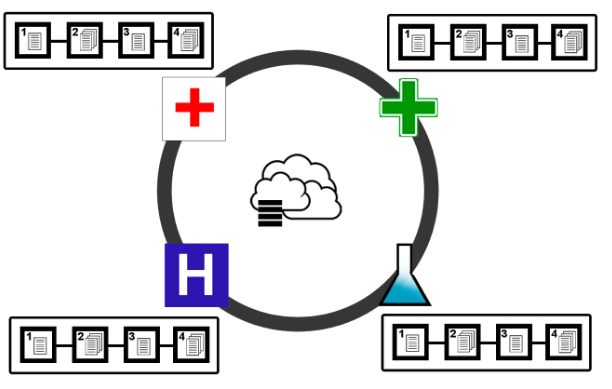
\includegraphics[width=0.7\linewidth]{imgs/interoperability.png}
\caption{\label{fig:interoperability}An Example of Interoperability with the
Blockchain Network} \end{figure}

The most simple case of an interaction in an Healthcare service is the
interaction between a patient and a doctor. In HLF this situation translates to
two organizations and two peers. Each peer belongs to an organization. One
organization represents the patients while the other represents the hospital
where the doctor works. 

To establish a communication between the two participating peers a channel can
be created ensuring information exchanged between the two on the channel is
private and does not exist on the rest of the network.  If a third organization
with another peer representing another health clinic joined the network then
another channel could be created between the patient's organization and this
new organization. If the patient were to insert his data into the channel then
the clinic would be able to view it everytime they wished. 

Starting in version 1.1 of Fabric the MSP allows Attribute Based Access Control
meaning access flow to the data can depend on the value of a certain attribute
of the certificate. Also it is possible to encrypt data and insert it into the
channel and then require a key to decrypt the data. In this case the patient
could give a key to the doctor to be able to access only his data. In the
current version of Fabric, version 1.2, private data collections were
introduced, meaning that some data can be marked as private on a channel while
other data can be public.

To conclude it was tought that to properly evaluate this solution a series of
experiments would be conducted. First some data would be present on the channel
when the user interacts that represents his identity in a certain clinic. The
patient would query the Blockchain for his data and receive his data if
everything worked accordingly. The second experiment was making the patient
share his data with the doctor in the channel. The last experiment consisted in
the patient trying to query data of another patient that was inserted at the
genesis of the network and seeing if the data was encrypted or was easily
readable. The outcomes of these experiments can shape the development of the
solution as it could take these results into consideration and highlight
possible problems.

\subsection{Implementation}

To create an interactive system that can manage the patients identity in an
Healthcare environment an application was built that the user interacts with.
Applications can be developed in any language as long as there is a Software
Development Kit (SDK) supporting the language. 

At the time of writing there is the Go language SDK and Node.js SDK available
with Go being the first programming language to get support and Java also being
added recently. 

After some research the Node.js SDK seemed to be on par with the Go one, in
regards to API and features. However, documentation was more sparse and harder
to find for the Node.js SDK. 

On the other hand Javascript seemed more approachable in contrast to Go, in
order to implement the system due to the author's familiarity with the Node.js
environment and with the Javascript programming language. Also, the application
and the smart contract could both be built in this language which was
considered an advantage as it simplifies dependency management. 

Ultimately, this application interfaces with smart contracts through the
Hyperledger Fabric Software Development Kit and the chaincode was built using
the Hyperledger Fabric Shim for Node.js and programmed in Javascript.

To avoid the need for multiple machines being used to form the network, a
Docker Compose file was used that defines, and orchestrates the main components
of the network through the Docker Engine. Each component consists in one or
more containers. Also, there is one  container defined to be used as a CLI to
interface with the network using the peer tool if needed for administrative
purposes. Docker was used as the containerization technology because it is
officially supported by Hyperledger and is currently the most popular
containerization tool.

To build the desired network configuration for the prototype, the configuration
file for the \textit{cryptogen} tool was edited to allow the network to have
two organizations, each of them with a peer associated. The configuration file
for the configtxgen tool was also edited to allow a channel of information
between the two organizations to be created. Each peer would serve as the
anchor peer~\footnote{Used to initiate communication between peers from
different organizations. The anchor peer serves as the entry point for another
organization’s peer on the same channel to communicate with each of the peers
in the anchor peer’s organization.} in each of the organizations.

An application was also built that allows for user enrollment to create a new
identity in the network. The application is run by a user and uses the
available SDK to call upon the operations that the smart contract makes
available. When a new user of the application enters the network, a function in
the smart contract initializes the creation of the patient's data and writes
the patient's Healthcare information to the ledger as a new asset and also
manages the ledger state through transactions as well as the world state.  The
overview of the architecture for this system is represented on Figure
\ref{fig:appOverview}. Due to the security mechanisms these transactions are
signed and endorsed by the administrator of the network and verified by the CA
servers.

\begin{figure}[ht] \centering
  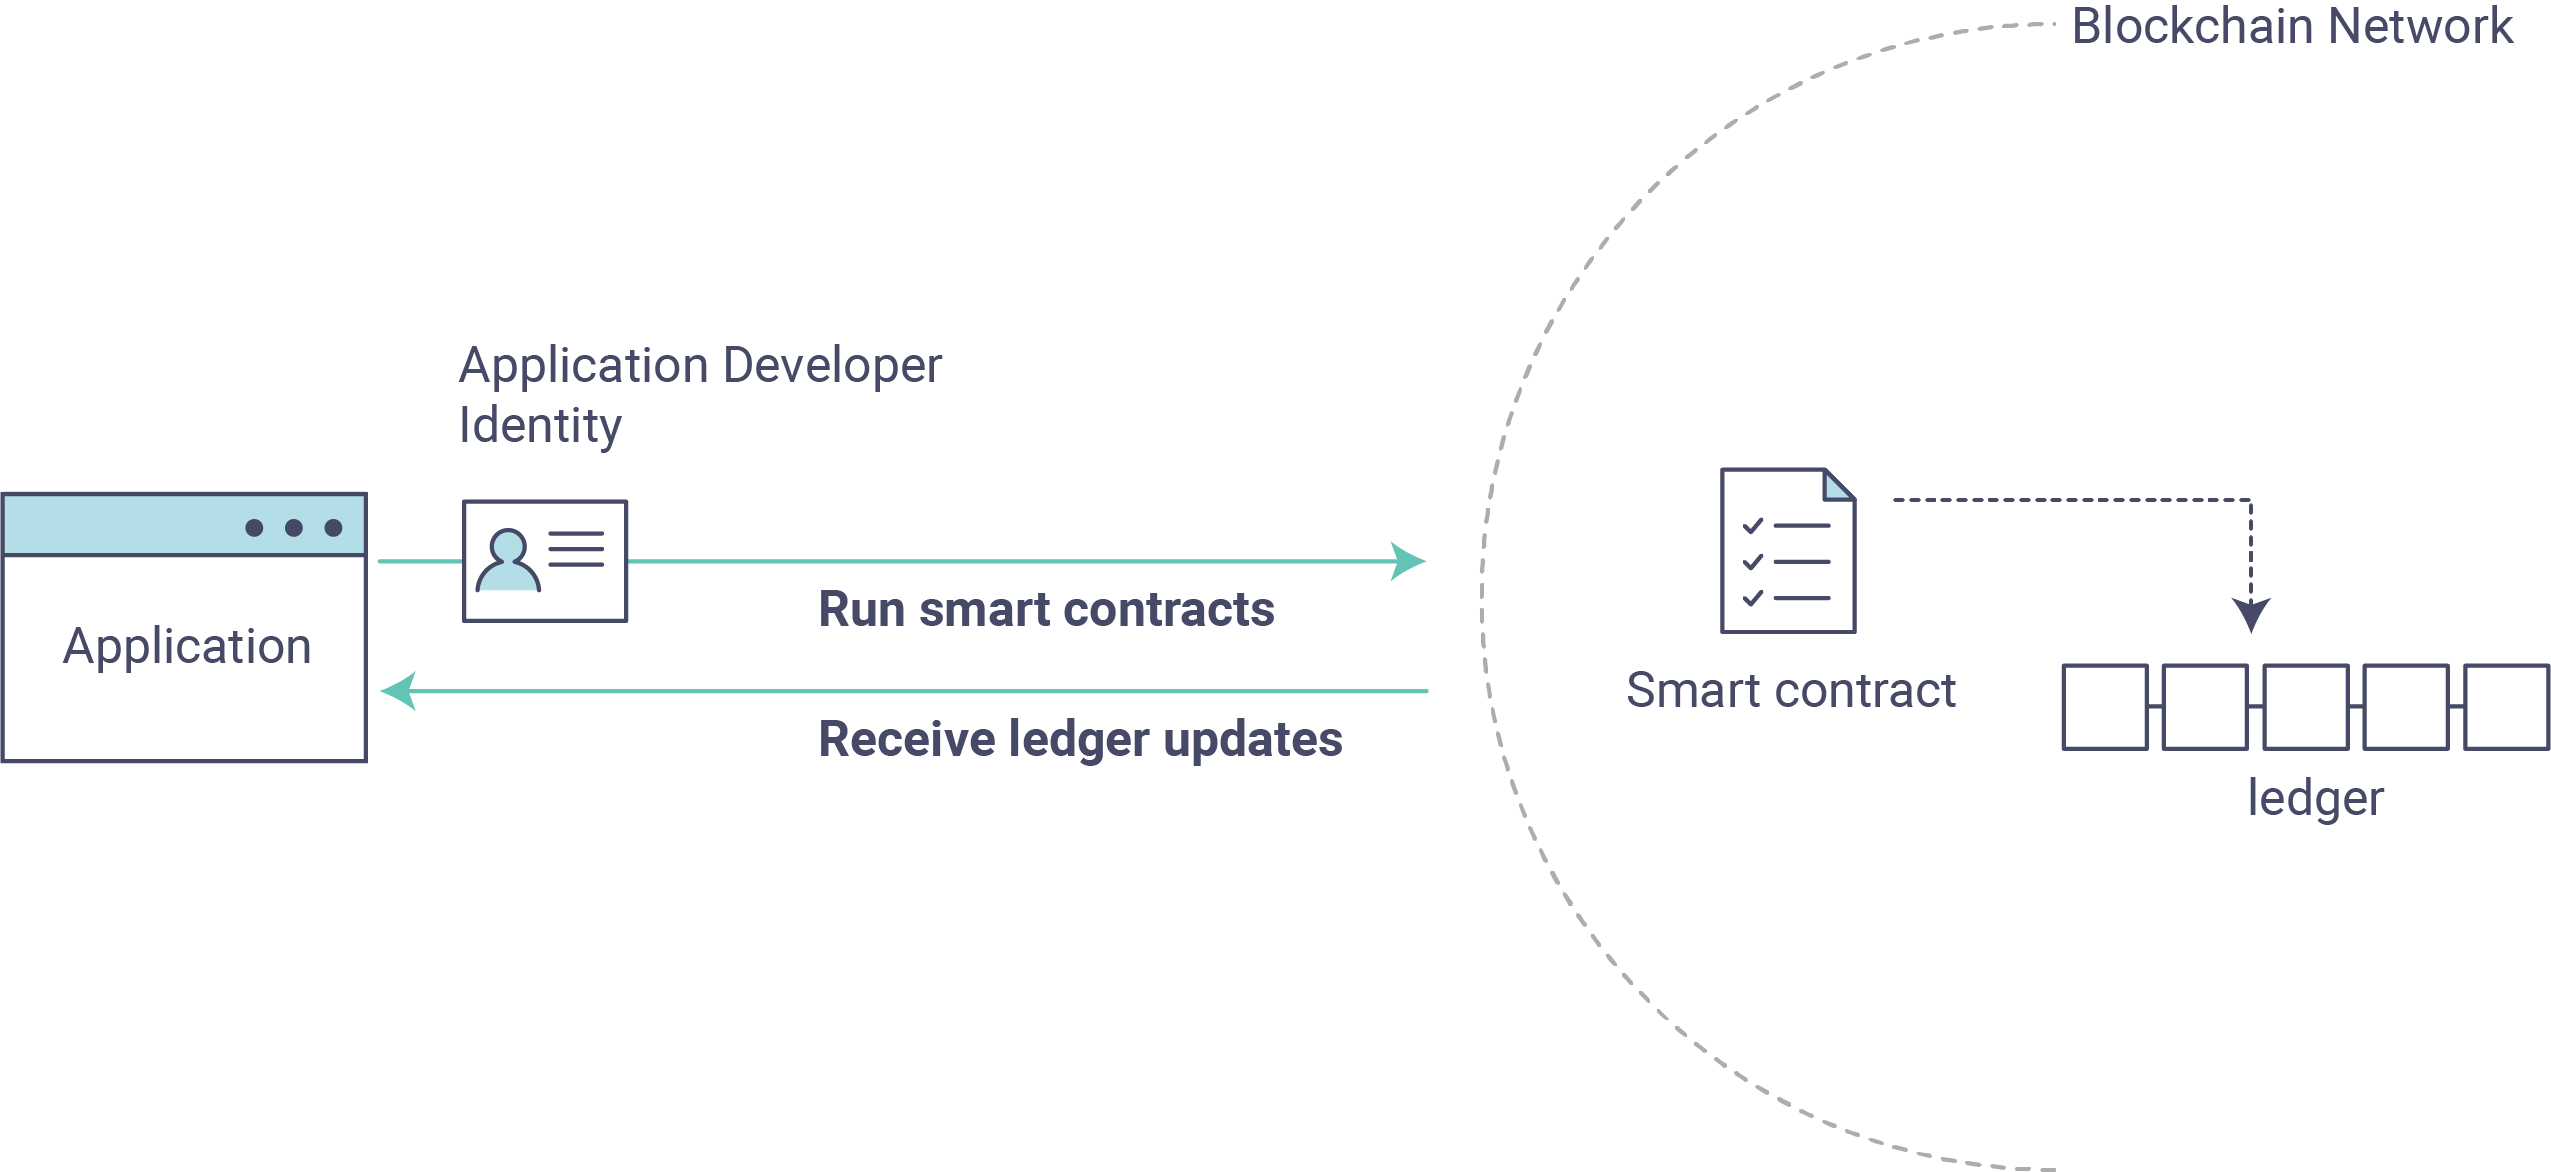
\includegraphics[width=1\linewidth]{imgs/hyperledgerAppOverview.png}
  \caption{\label{fig:appOverview}An Overview of the System Architecture
  (Source:
  \href{http://hyperledger-fabric.readthedocs.io/en/latest/write_first_app.html}{HLF
  Fabric Documentation})} 
\end{figure}

The assets loaded contain the necessary fields to identify a patient in an
Healthcare context, such as its name and birth date, for example, as well as
some other information necessary to manage this data as discussed previously.

These operations form an Application Programming Interface (API) as seen in
Figure~\ref{fig:smartContractOverview} that returns a payload in JSON format
with information from the network. This API allows a query to be made to the
network that returns the patients information, changing incorrect or outdated
information or disabling the identity structure of someone who is not
participating in the network actively anymore in order for that information to
be read-only from that point on, for example, with more available. This system
architecture leads to a modular as well as extensible approach regarding the
availability of new operations that become available as soon as new versions of
the smart contract are deployed.  

\begin{figure}[ht] 
  \centering
  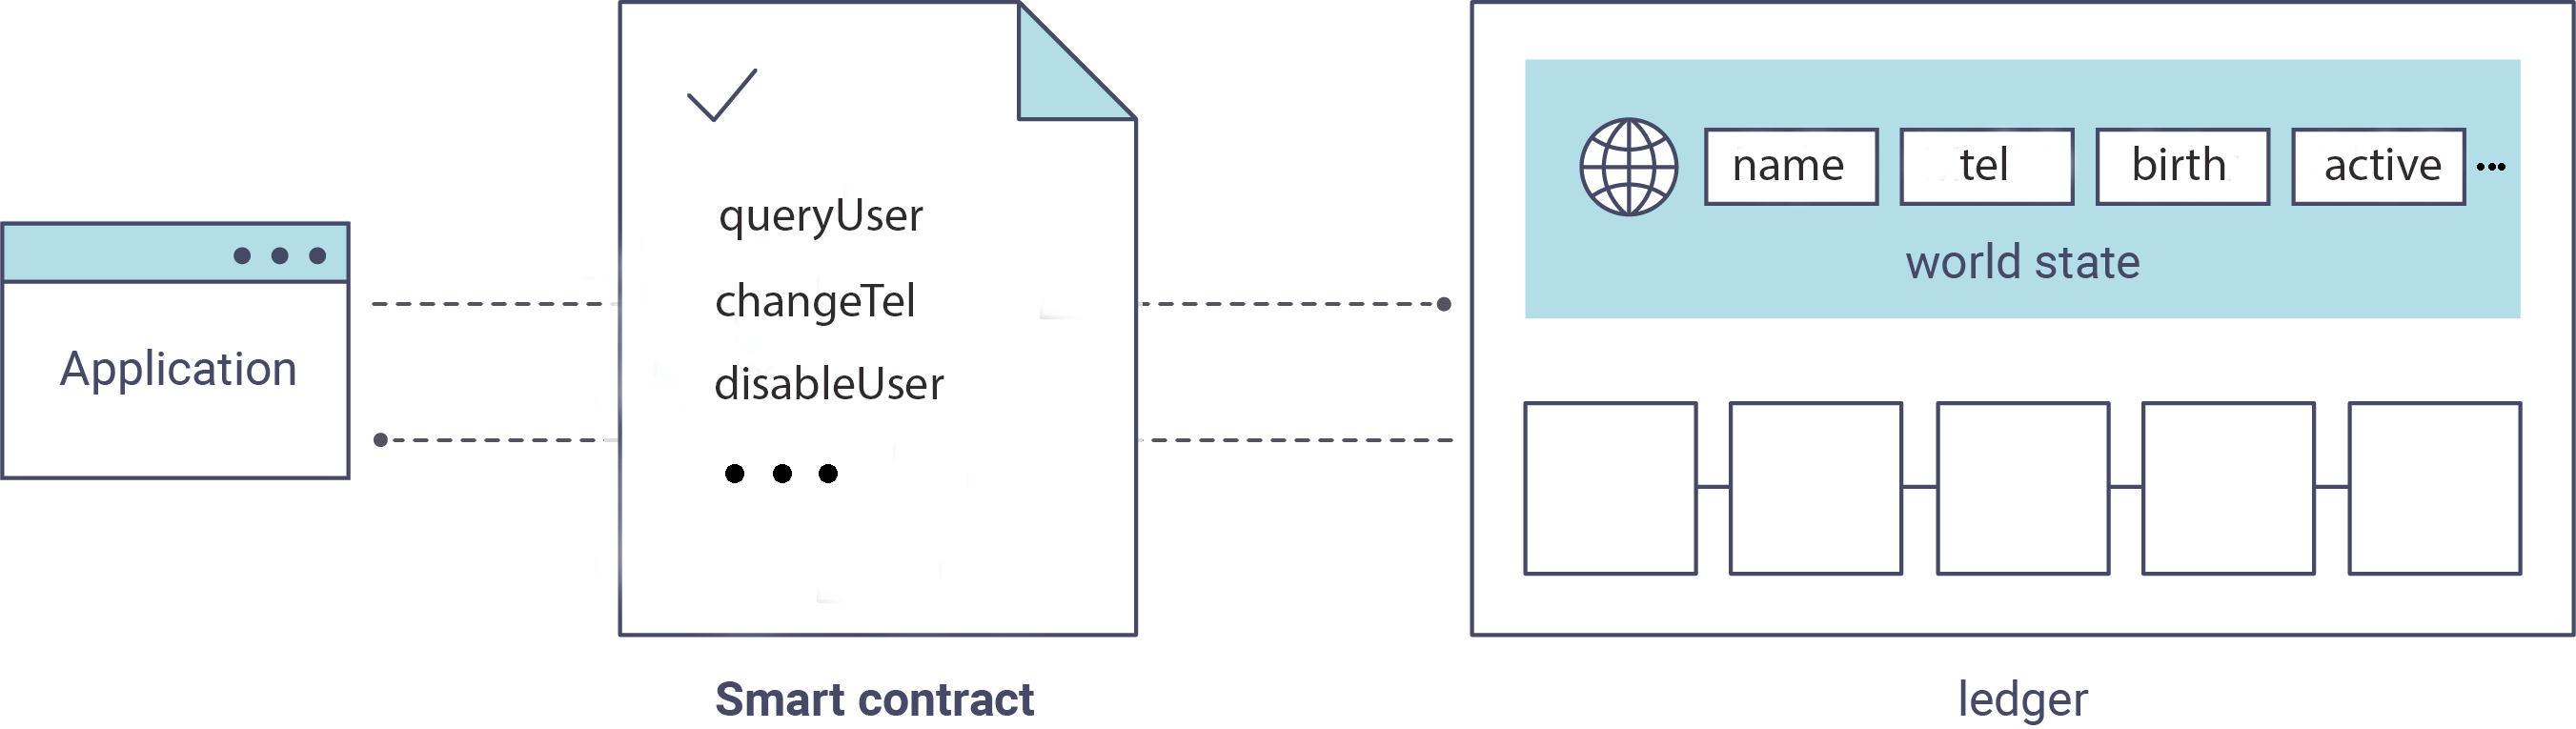
\includegraphics[width=1\linewidth]{imgs/smartContractOverview.png}
  \caption{\label{fig:smartContractOverview}Smart Contract Operations Example
  (Original:
  \href{http://hyperledger-fabric.readthedocs.io/en/latest/write_first_app.html}{HLF
  Fabric Documentation})} 
\end{figure}

The network was brought up using the Docker Compose technology and an
administrator was enrolled into the network. This step is required because
every action must be verified through a chain of trust and the administrator is
the root CA in the network.

The next step was registering the patient and the doctor. Both the patient and
the doctor ran the register function of the application and were asked for a
password. After successfully registering they were show their assigned patient
number and the password was stored in the certification as well as the patient
number assigned to them. At this point they became active participants in the
network. In this case the assets that represent their identity were not created
because they had exceptionally been created before hand by the administrator to
simplify the process. The normal flow would be the respective asset creation on
registration.

\section{Testing and Adjusting the System}

With the network in place and the peers set up and registered the experiments
proposed have now their requirements fulfilled.

\subsection{Experiments}

The patient used the function provided by the application to query the network
for his information. He searched for his patient number and was shown his
information successfully. This shows that the information was recorded with
success when the chaincode was deployed. The simple way to query personal
information with an assigned patient number also proved successful and shows
that this system can be used to store patient's identity data and retrieve it.

Then the patient had to share his information with the doctor. To do this it
was necessary to assume that the patient had given his patient number to the
doctor so that he could use the application built to query for that patient
number. The doctor queried the network for the patient's information and was
able to access it successfully. This proves that this platform allows
surprisingly, to very easily share information between a patient and a doctor
using a smart contract in a simple way.

Finally the patient tried to access another patient's data. It was necessary to
assume that he was given the patient number by the respective patient. When he
queried the network for that patient's data it became clear what already had
arose suspicions in the previous experiments. He was actually able to access
that data without a problem. This would be okay if the number was willingly
given to him. However if the number was obtained unwillingly it could prove a
problem. This meant that the solution currently, did not meet the requirement
of the information being confidential that was defined previously, even tough
it is transparent and has high availability since the information was spread
through multiple peers and could be on multiple channels. It became clear that
some additional data security measures was needed.

\subsection{Encrypting Data}

To make information confidential some form of obfuscation or encryption could
be used. Fabric also features Attribute Based Access Control meaning that the
chaincode logic could be altered to check if some attribute was present on the
doctor's certificate that indicated that he had access to certain patients
information. This could work for application users however if users used some
tool like Hyperledger Explorer they could see the data since the data is stored
as a plain text.

After investigating the different possibilities and making some tests it was
decided to use encryption. The flow of the operations would be simple. When the
patient's data was registered he would receive a notification of a data key and
the data would be encrypted using for example a traditional SHA-256 encryption
algorithm. The data would be encrypted using symmetric key encryption with the
generated key being stored on the X.509 securely.  If the patient wanted to
share his information with with someone he would give him the key and that
would allow him to decrypt the encrypted patient's data.  To complete this
system the key should expire after a certain amount of time and refresh itself.

With this system in place the last requirement was fulfilled and the system is
now considered to be reasonable for the purposes of this thesis. At this point
it is reasonable to evaluate this solution as an identity management platform
in the Healthcare context.

\section{Evaluation and a Review of Thesis Goals}

This solution was evaluated against the international standard for information
security known as the CIA triad model, in order to draw further conclusions and
evaluate how secure the built system is in regards to its information which is
a critical concern in this field. The three pillars that form this standard are
the preservation of the confidentiality, ensuring information integrity and
information availability.

\subsection{Confidentiality}

Confidentiality of the information stored in the network was considered a key
requirement when the requirements were presented. The Hyperledger Fabric was a
prime candidate for building the solution upon due to its focus on privacy and
a more enterprise approach to Blockchain development. While it offers many
features such as channels that truly do segregate information in a way that
many equivalent platforms cannot do at the moment it is also true that by
default data will be stored in plain text. 

To solve this problem it was necessary to implement data encryption on top of
the network using chaincode. This way even if someone was able to access the
underlying database or if someone used a tool like Hyperledger Explorer to
explore the network all it would see is encrypted data that would require a key
to encrypt. With these considerations in mind it, even tough there are a number
of aspects that define confidentiality it can be said that the built system
provides a confidential data storage.

\subsection{Integrity}

One of the key aspects of a Blockchain system is the immutability of data. This
means that once information is written it cannot be changed or erased. The
transaction logs assure that the specific version of that asset is recorded
permanently in the network. In order to comply with privacy regulations some
data can become only visible as an hash but it still remains there. Therefore
the integrity of data on this Blockchain platform and solution is also
preserved.

\subsection{Availability}

Even tough Fabric is a permissioned Distributed Ledger Platform and as such it
is administrated by an administrator it is also distributed and therefore
avoids having a single point of attack. By default it is more available than a
simple informational system that is centralized. In this aspect it can be said
the more the network scales, the more robust it becomes and therefore more
availability it provides as information redundancy also increases.

\subsection{Thesis Goals}

The goal of this thesis was to evaluate if a system could be built based on
Blockchain technology to manage the patients identity in the Healthcare
environment. Using Hyperledger Fabric a system was built that successfuly can
create, manage and delete patients data. Information can be shared in a secure
manner and interoperability eases organization into adopting this system. This
system provides benefits to the medical staff as well as the patients due to
transparency in how data is handled and secured.

However the costs of deploying this system in a production ready environment
would be higher compared to a more traditional approach. Since this system is
build upon a Permissioned Platform, machines to host the central services need
to be acquired and an administrator of the platform is necessary for the
necessary maintenance. As the network grows it would become more resilient and
additional servers could be used to expand the core availability of Blockchain
components.

There is also the question of scalability. Even tough a Permissioned Blockchain
is always faster in relation to a Permissionless variant it still is far from
matching the scalability and performance of the Electronic Payment Management
System created by SIBS for banking transactions, for example. If this system
was intended for global use then additional approaches would need to be taken
regarding this matter.

With this said the pace of development has been relatively fast with new
releases on a quarterly basis that focus on the issues of scalability and
privacy, two important features pertaining to the system this Thesis proposed.

}
%
% ----------------------------------------------------------------
%
%	APÊNDICES
%
%	Texto complementar da tese.
%
\tueAPENDICES % Material de suporte
{
	%!TEX root = main.tex
\chapter{Bases Formais}

Lorem ipsum dolor sit amet, consectetur adipiscing elit. Vivamus vitae est vitae risus varius malesuada et eget velit. Morbi tincidunt venenatis tellus, in volutpat ante varius et. Fusce congue maximus velit ac dignissim. Integer hendrerit pharetra libero, at vehicula odio vestibulum eget. Etiam eget fringilla leo, sit amet posuere nisl. Aenean at tincidunt felis. Cras rhoncus mauris libero, a vestibulum \index{risus} faucibus quis. Aenean malesuada vitae nibh ut dapibus. Pellentesque vel blandit odio.

Maecenas massa leo, egestas id augue at, aliquam iaculis leo. Etiam ac lacus tempus, malesuada dolor vel, mattis leo. Duis tortor mi, accumsan vitae ligula eu, luctus accumsan diam. Etiam venenatis elit non magna aliquam eleifend. Phasellus in nunc at arcu iaculis ultrices sed sed ante. Nullam in velit a metus convallis vestibulum a vitae turpis. Proin fringilla dui tempor, ultrices metus nec, lobortis elit. Sed at posuere augue. Phasellus ac massa fringilla, convallis urna nec, aliquet orci. Mauris placerat tellus vel scelerisque tempus. Donec lacinia tincidunt mattis. Donec congue, augue sed ullamcorper placerat, erat nunc vestibulum tellus, vel consequat sem diam in magna. Vivamus ac dolor lacinia magna pharetra maximus. Nulla congue feugiat vehicula. Praesent luctus purus ac justo tempor eleifend.

Nunc eu ex vel ipsum ultrices molestie. In eget sodales turpis. Donec egestas facilisis nulla id feugiat. Duis \index{gravida} lorem quis porttitor interdum. Sed turpis leo, aliquet non metus a, vulputate volutpat ante. Donec neque metus, volutpat quis congue non, aliquam sed nunc. Curabitur erat mauris, elementum id rhoncus quis, condimentum eu felis. Quisque porta gravida velit a congue. Nulla gravida suscipit pulvinar. Sed sed erat ut turpis consequat sagittis. Sed scelerisque, massa ac tincidunt rutrum, libero dolor suscipit lorem, interdum dignissim massa enim a purus. Aliquam porta orci non urna sollicitudin, sed lobortis nibh ullamcorper. Aliquam erat volutpat. Phasellus ac purus in massa aliquet ultricies non sit amet justo.

Quisque placerat lobortis risus. Vestibulum ante ipsum primis in faucibus orci luctus et ultrices posuere cubilia Curae; Pellentesque eget odio sed lectus sollicitudin consectetur et ornare libero. Aliquam et ullamcorper arcu. Fusce mollis euismod purus, vitae auctor quam lobortis eu. Nunc mollis, velit eu cursus feugiat, nunc neque pellentesque arcu, a suscipit tellus nunc quis quam. Cras diam est, fermentum a rutrum sed, pretium eu tortor.

Integer imperdiet, est mattis imperdiet luctus, nunc nisl sodales justo, sit amet dapibus urna mauris sit amet diam. Donec et massa lectus. Cras nec pellentesque odio. Integer porta varius enim vel ornare. Donec nec commodo dui, a aliquet \index{magna}. Vestibulum sollicitudin nibh justo, ac mattis nibh volutpat et. Morbi eget condimentum enim, sit amet lobortis ligula. Vivamus nec mauris purus.
	%!TEX root = main.tex
\chapter{Resultados Empíricos}

Lorem ipsum dolor sit amet, consectetur adipiscing elit. Vivamus vitae est vitae risus varius malesuada et eget velit. Morbi tincidunt venenatis tellus, in volutpat ante varius et. Fusce congue maximus velit ac dignissim. Integer \index{hendrerit} pharetra libero, at vehicula odio vestibulum eget. Etiam eget fringilla leo, sit amet posuere nisl. Aenean at tincidunt felis. Cras rhoncus mauris libero, a vestibulum risus faucibus quis. Aenean malesuada vitae nibh ut dapibus. Pellentesque vel blandit odio.

Maecenas massa leo, egestas id augue at, aliquam iaculis leo. Etiam ac lacus tempus, malesuada dolor vel, mattis leo. Duis tortor mi, accumsan vitae ligula eu, luctus accumsan diam. Etiam venenatis elit non magna aliquam eleifend. Phasellus in nunc at arcu iaculis ultrices sed sed ante. Nullam in velit a metus convallis vestibulum a vitae turpis. Proin fringilla dui tempor, ultrices metus nec, lobortis elit. Sed at posuere augue. Phasellus ac massa fringilla, convallis urna nec, aliquet orci. Mauris placerat tellus vel scelerisque tempus. Donec lacinia tincidunt mattis. Donec congue, augue sed ullamcorper placerat, erat nunc vestibulum tellus, vel consequat sem diam in magna. Vivamus ac dolor lacinia magna pharetra maximus. Nulla congue feugiat vehicula. Praesent luctus purus ac justo tempor eleifend.

Nunc eu ex vel ipsum ultrices molestie. In eget sodales turpis. Donec egestas facilisis nulla id feugiat. Duis gravida lorem quis porttitor interdum. Sed turpis leo, aliquet non metus a, vulputate volutpat ante. Donec neque metus, volutpat quis congue non, aliquam sed nunc. Curabitur erat mauris, elementum id rhoncus quis, condimentum eu felis. Quisque porta gravida velit a congue. Nulla gravida suscipit pulvinar. Sed sed erat ut turpis consequat sagittis. Sed scelerisque, massa ac tincidunt rutrum, libero dolor suscipit lorem, interdum dignissim massa enim a purus. Aliquam porta orci non urna sollicitudin, sed lobortis nibh ullamcorper. Aliquam erat volutpat. Phasellus ac purus in massa aliquet ultricies non sit amet justo.

Quisque placerat lobortis risus. Vestibulum ante ipsum primis in faucibus orci luctus et ultrices posuere cubilia Curae; Pellentesque eget odio sed lectus sollicitudin consectetur et ornare libero. Aliquam et ullamcorper arcu. Fusce mollis euismod purus, vitae auctor quam lobortis eu. Nunc mollis, velit eu cursus feugiat, nunc \index{neque} pellentesque arcu, a suscipit tellus nunc quis quam. Cras diam est, fermentum a rutrum sed, pretium eu tortor.

Integer imperdiet, est mattis imperdiet luctus, nunc nisl \index{sodales} justo, sit amet dapibus urna mauris sit amet diam. Donec et massa lectus. Cras nec pellentesque odio. Integer porta varius enim vel ornare. Donec nec commodo dui, a aliquet magna. Vestibulum sollicitudin nibh justo, ac mattis nibh volutpat et. Morbi eget condimentum enim, sit amet lobortis ligula. Vivamus nec mauris purus.
}
%
% ----------------------------------------------------------------
%
%	BIBLIOGRAFIA
%
%
\tueBIBLIOGRAFIA{
  \bibliographystyle{alpha}
  \bibliography{bibliography.bib}
}
%
% ----------------------------------------------------------------
%
%	ÍNDICE REMISSIVO
%
%\tueINDICEREMISSIVO{}
%
% ----------------------------------------------------------------
%
% ================================================================
%
%	Modo ORGANIZAÇÃO DA DISSETAÇÃO COMPLETA.
%
%	Prevê que
%		- a informação sobre título, autor, orientadores, etc está definida acima e que
%		- a obra tem a seguinte estrutura:
%
%			prefácio
%			agradecimentos
%			tabela de conteúdos
%			lista de figuras
%			lista de tabelas
%			lista de acrónimos
%			sumário
%			tradução do sumário
%			------------------------------
%			CONTEÚDO (vários capítulos)
%			APÊNDICES (vários capítulos)
%			------------------------------
%			bibliografia
%			índice remissivo
%
% ================================================================
%
\tueDOCUMENTO
%
% ================================================================
%	Modo CAPA, CONTRA-CAPA e LOMBADAS.
%
%	Prevê que a informação sobre título, autor, orientadores, etc está definida acima.
%
% ================================================================
%
%\tueCAPAS

